\documentclass[11pt]{jarticle}
\usepackage{graphicx}
\begin{document}
\begin{center}
工学基礎実験実習 レポート

学生番号09501527 重近 大智

レポート提出期限 : 2019/05/14
\end{center}
\section{課題1}
Windowsの人気度(一般人100人に調査)

*Microsoft社の調査とは関係ありません。

\begin{tabular}{|c|c|c|}
\hline
      &好き&嫌い\\
\hline
Windows 10&10&90\\

Windows 8.1&30&70\\

Windows 7&99&1\\
\hline

\end{tabular}
\section{課題2}
\begin{center}
\large \em 問題
\end{center}
1、次の関数の偏導関数$z_x ,z_y$を求めよ。
\begin{center}

\begin{equation}
z=\frac{y}{x}+\frac{x}{y}
\end{equation}
\end{center}

2、次の定積分の値を求めよ。
\begin{center}
\begin{equation}
\int_0^π {\sin x \cos xdx}
\end{equation}
\end{center}
\section{課題3}
集合演算に補集合がある。$A$の補集合を$A^c$と書く。$A^c$は$A$に含まれない要素からなる集合である。形式的に定義すると次のようになる。ただし、「左辺=def右辺」は左辺が右辺によって定義されることを表す。よく使われる集合演算は和、積、差である。形式定義はそれぞれ以下の通りである。

$\bullet$ 補集合 $A^c$=def$\{x|x \notin A\}$

$\bullet$ 和 $A \cup B$=def$\{x|(x \in A)あるいは(x \in B)\}$

$\bullet$ 積 $A \cap B$=def$\{x|(x \in A)かつ(x \in B)\}$

$\bullet$ 差 $A-B$=def$\{x|(x \in A)かつ(x \notin B)\}$
\section{課題4 2進数と10進数の対応表}
2進数と10進数の対応表
プログラム(bindec.c)を以下に示す。
\begin{verbatim}
     1	main(){
     2	  int i,j,k,l,p=0;
     3	  printf("2進数\t10進数\n");
     4	  for(i=0;i<2;i++)
     5	    for(j=0;j<2;j++)
     6	      for(k=0;k<2;k++)
     7		for(l=0;l<2;l++){
     8		  printf("%d%d%d%d\t%d\n",i,j,k,l,p++);
     9		}
    10	}

実行結果を以下に示す。

2進数	10進数
0000	0
0001	1
0010	2
0011	3
0100	4
0101	5
0110	6
0111	7
1000	8
1001	9
1010	10
1011	11
1100	12
1101	13
1110	14
1111	15

\end{verbatim}

\section{図の挿入(LibreOffice Draw)}
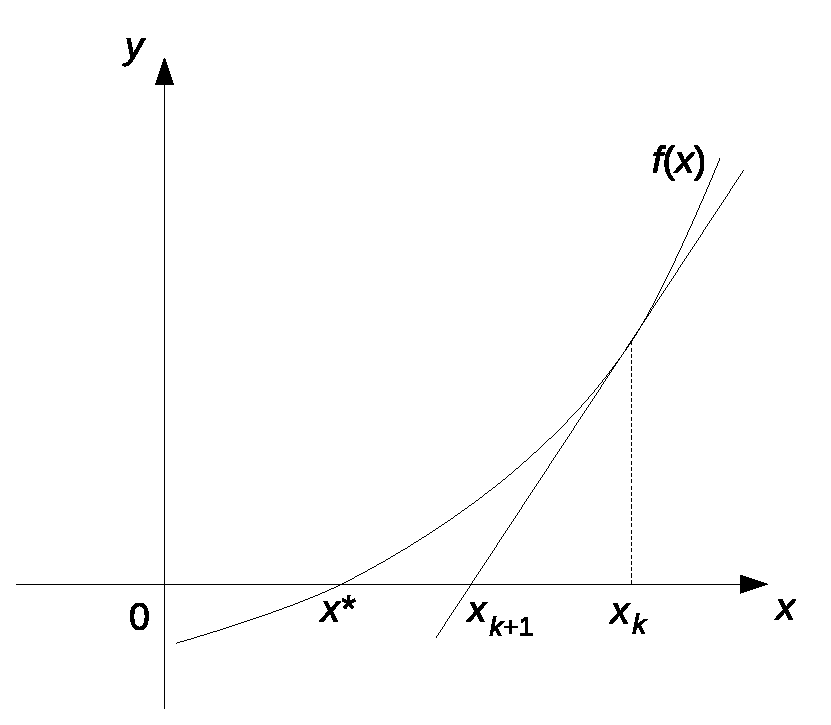
\includegraphics{figure2.eps}

\section{図の挿入(GNUPLOT)}
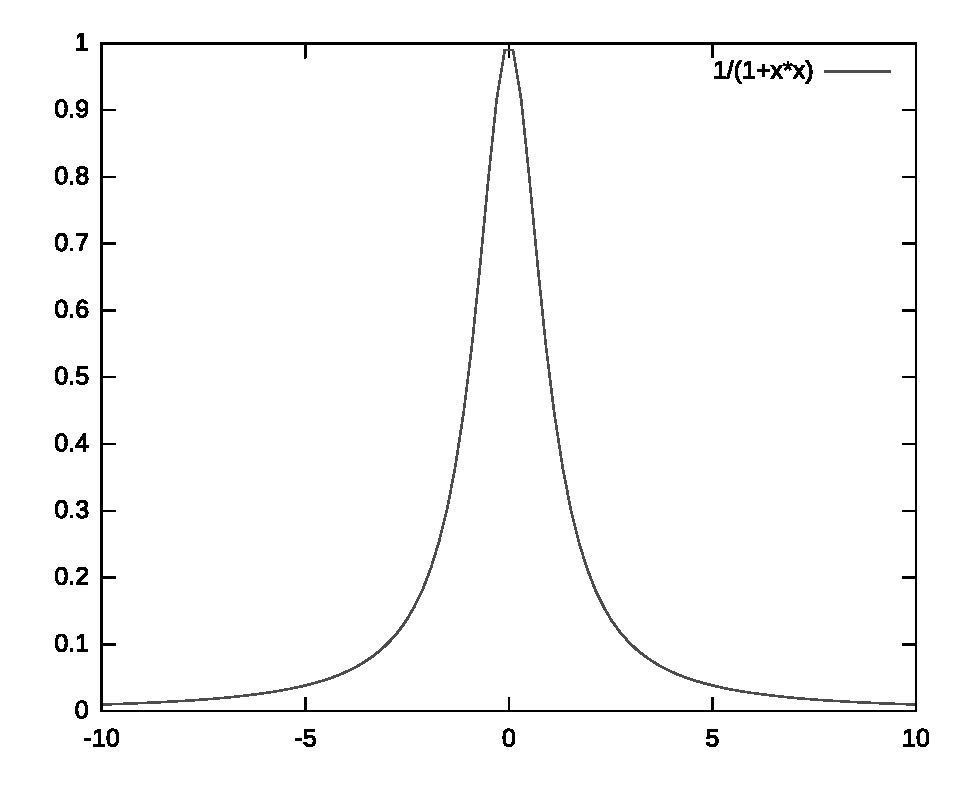
\includegraphics{figure3.eps}

\section{図の作成(\LaTeX)}
\begin{picture}(130,70)
\put(5,5){\line(1,0){120}}
\put(125,5){\line(-1,1){60}}
\put(65,65){\line(-1,-1){60}}
\put(65,5){\circle{40}}
\put(125,5){\line(-1,-1){60}}
\put(5,5){\line(1,-1){60}}
\end{picture}
\\
\\
\\

\section{前回からの修正点}
課題3のitemizeコマンドによる黒点をbulletコマンドによる表示に変更した。
\end{document}
